%% 
%% File:    PResCnam-final.tex
%% Author:  Stefano Secci (stefano.secci@lecnam.net)
%% Adapté pour le projet CNAM
%% 

\documentclass[a4paper,12pt]{article}

\usepackage[francais]{babel}
\usepackage{fancyhdr}
\usepackage[utf8]{inputenc}
\usepackage[T1]{fontenc}
\usepackage{epsfig}
\usepackage{calc}
\usepackage{url}
\usepackage{boxedminipage}
\usepackage{graphicx}
\usepackage{hyperref}

%%%%%%%%%%%%%%%%%%%%%%%%%%%%%%%%%%%%%%%%%%%%%%%%%%%%%%%%%%%
%% Définitions à personnaliser 

%%%% Indiquer le nom de l'encadrant ci-dessous:
\def\nomEncad{Y. ~Benchaïb} % 

%%%% Indiquer les noms des étudiants participant ci-dessous:
\def\nomEtudA{J.~Mootooveeren}
\def\nomEtudB{A.~Atmane}
\def\nomEtudC{A.~Landois}
\def\nomEtudD{J.~Montguillon}

%%%% Indiquer la référence (numero) et le nom du sujet ci-dessous:
\def\refProjet{2} 
\def\titreProjetCourt{Tetragon \& eBPF IDS}
\def\titreProjetLong{Observabilité et graphes de comportement avec Tetragon pour des attaques zero-day}

\def\typeDoc{Rapport Final}
 
%%%%%%%%%%%%%%%%%%%%%%%%%%%%%%%%%%%%%%%%%%%%%%%%%%%%%%%%%%%
%% Définitions à ne pas modifier
 
\setlength{\voffset}{-1in} 
\setlength{\topmargin}{15mm}         
\setlength{\headheight}{20mm}        
\setlength{\headsep}{10mm}            
\setlength{\textheight}{220mm}       
\setlength{\footskip}{12mm}          

\setlength{\hoffset}{-1in} 
\setlength{\oddsidemargin}{25mm}     
\setlength{\evensidemargin}{25mm}    
\setlength{\marginparwidth}{0mm}     
\setlength{\marginparsep}{0mm}       
\setlength{\textwidth}{160mm}        

\def\annee{2026} % 

\begin{document}
\selectlanguage{francais}

%%%%%%%%%%%%%%%%%%%%%%%%%%%%%%%%%%%%%%%%%%%%%%%%%%%%%%%%%%%
%% Définition des en-têtes et pied de pages
\pagestyle{fancyplain}
\lhead[\fancyplain{}{\texttt{Conservatoire national des arts et métiers}\\
          UE \textbf{USRS7N} Mars \annee \\ \nomEncad}]
      {\fancyplain{}{\textsc{Conservatoire national des arts et métiers}\\
          UE \textbf{USRS7N} Mars \annee \\ \nomEncad}}
\chead[\fancyplain{}{\textbf{Projet \refProjet\\\titreProjetCourt}}]
      {\fancyplain{}{\textbf{Projet \refProjet\\\titreProjetCourt}}}
\rhead[\fancyplain{}{\nomEtudA\\\nomEtudB\\\nomEtudC\\\nomEtudD}]
      {\fancyplain{}{\nomEtudA\\\nomEtudB\\\nomEtudC\\\nomEtudD}}
\lfoot[\fancyplain{}{\includegraphics[width=3cm]{logo-cnam.png}}]
      {\fancyplain{}{\includegraphics[width=3cm]{logo-cnam.png}}}
\cfoot[\fancyplain{}{\textbf{\thepage/\pageref{fin}}}]
      {\fancyplain{}{\textbf{\thepage/\pageref{fin}}}}
\rfoot[\fancyplain{}{\typeDoc}]
      {\fancyplain{}{\typeDoc}}

%%%%%%%%%%%%%%%%%%%%%%%%%%%%%%%%%%%%%%%%%%%%%%%%%%%%%%%%%%%

~

\begin{center}
  \begin{boxedminipage}{14cm}{
      \begin{center}
        ~\\\LARGE\textbf{\titreProjetLong}\\
        ~\\\large Encadrant: \textbf{\nomEncad}\\
        ~\\\large Etudiants: \textbf{\nomEtudA, \nomEtudB, \nomEtudC, \nomEtudD}\\
        ~
      \end{center}
      }
  \end{boxedminipage}
\end{center}

~

\tableofcontents

\newpage

\section{Cahier des charges}

L’émergence des architectures cloud-native et des environnements conteneurisés complexifie la sécurisation des systèmes d’information. Face à la sophistication des cybermenaces, notamment les attaques zero-day exploitant des vulnérabilités inconnues, les systèmes de détection d’intrusion (IDS) traditionnels basés sur des signatures atteignent leurs limites. Il est crucial de mettre en place des mécanismes d’analyse comportementale proactifs, capables de détecter des anomalies même en l’absence de signatures connues.

Ce projet vise à concevoir, déployer et évaluer une solution de détection d’intrusion basée sur la modélisation de graphes comportementaux, exploitant eBPF (Extended Berkeley Packet Filter) pour l’observabilité sécurisée au niveau du noyau Linux. L’outil principal sera Tetragon, permettant la capture d’événements système et réseau sans modification du noyau.

Les besoins fonctionnels incluent la détection en temps réel des comportements suspects, la génération et le traitement d’événements JSON, ainsi que la création de graphes de comportement liant pods, processus, fichiers et connexions réseau. Les besoins non fonctionnels concernent la performance, la compatibilité avec Kubernetes et la sécurité du système de monitoring.

Les principales parties prenantes sont les administrateurs systèmes et les équipes de sécurité des environnements cloud-native. Le projet ne couvrira pas les environnements Windows ni les attaques réseau nécessitant des techniques avancées de machine learning.

Le projet se structurera en quatre tâches principales : (1) réalisation d’un état de l’art sur eBPF, observabilité cloud-native et graphes pour la cybersécurité ; (2) étude approfondie de Tetragon et de ses TracingPolicies ; (3) développement d’une chaîne d’outils Python pour transformer les événements JSON en graphes de comportement ; (4) déploiement d’un environnement virtuel Linux/Kubernetes pour simuler scénarios légitimes et attaques et évaluer l’efficacité de la solution.

\section{Plan de développement}

\subsection{Introduction}

Ce projet vise à concevoir une plateforme de détection d’anomalies zero-day dans un environnement Kubernetes, en exploitant l’observabilité bas niveau offerte par eBPF. L’objectif scientifique est d’évaluer si la modélisation des comportements système sous forme de graphes dynamiques permet d’identifier des activités malveillantes inédites sans signature préalable.

L’architecture repose sur la collecte d’événements noyau via Tetragon, leur transformation en structures exploitables, puis leur analyse algorithmique pour détecter des déviations comportementales. Le développement est structuré en quatre tâches progressives couvrant cadrage, implémentation, validation et consolidation.

\subsection{Tâche 1 : Cadrage scientifique et architectural}

Cette première phase établit les bases conceptuelles et techniques. Elle comprend une étude approfondie d’eBPF et du fonctionnement de Tetragon en environnement Kubernetes (déploiement DaemonSet, TracingPolicies). Un état de l’art sur la détection d’anomalies basée sur graphes est réalisé, ainsi qu’une analyse des scénarios d’attaque inspirés du framework MITRE ATT\&CK.

Les livrables incluent un cahier des charges détaillé, un schéma d’architecture globale (collecte, traitement, stockage, analyse) et un planning précis. Cette phase garantit la cohérence scientifique et la faisabilité technique du projet.

\subsection{Tâche 2 : Implémentation de l’infrastructure et du pipeline}

Cette phase correspond au cœur du développement. L’infrastructure Kubernetes est déployée localement afin d’héberger Tetragon et les composants applicatifs. Les événements système collectés sont transformés en graphes dynamiques à l’aide de NetworkX.

Un pipeline Python assure l’ingestion, la normalisation et la mise à jour continue des graphes comportementaux. Un modèle de référence (baseline) représentant le comportement normal est construit. Des métriques d’évaluation sont définies : précision, rappel et taux de faux positifs. Cette étape permet d’obtenir un prototype fonctionnel.

\subsection{Tâche 3 : Validation expérimentale et tests offensifs}

La troisième phase consiste à évaluer la robustesse du système. Des scénarios d’attaque contrôlés (reverse shell, élévation de privilèges, exfiltration) sont exécutés afin d’observer la capacité du modèle à détecter des déviations.

Une analyse quantitative est menée à partir des métriques définies précédemment. Les cas de non-détection sont étudiés afin d’identifier les limites structurelles du modèle et d’améliorer les critères de comparaison de graphes.

\subsection{Tâche 4 : Optimisation et finalisation}

La dernière phase vise l’optimisation des performances (complexité des graphes, latence d’analyse) et l’amélioration de la visualisation via un tableau de bord interactif. Le code est documenté pour garantir la reproductibilité. Le rapport final consolide l’ensemble des résultats expérimentaux et des choix méthodologiques.


\section{État de l'art}

Dans un contexte technologique où les architectures monolithiques cèdent la place aux microservices orchestrés par des solutions comme Kubernetes, les surfaces d'attaque se sont démultipliées. La sécurité périmétrique classique est devenue insuffisante, imposant l'adoption de stratégies de sécurité dites \textit{Zero Trust} et nécessitant une observabilité au plus près du système d'exploitation. Cette section dresse un panorama des technologies sous-jacentes à notre projet, en détaillant eBPF, les concepts d'observabilité avec Tetragon, et l'application de la théorie des graphes à la détection de menaces zero-day.

\subsection{Fondements et évolution d'eBPF}
La technologie BPF (\textit{Berkeley Packet Filter}) a été initialement conçue en 1992 pour le filtrage de paquets réseau de manière performante. Cependant, depuis 2014, le noyau Linux a intégré une version profondément remaniée : eBPF (\textit{Extended BPF}) \cite{gbadamosi2024ebpf}. 

Souvent comparé à ce que JavaScript représente pour les navigateurs web, eBPF permet d'exécuter des programmes personnalisés au sein même du noyau Linux, sans avoir à modifier le code source de ce dernier ni à charger des modules additionnels (LKM - \textit{Linux Kernel Modules}), historiquement sources d'instabilités et de failles de sécurité \cite{vieira2020fast}. La sécurité de l'hôte est garantie par un composant clé : le vérificateur (\textit{verifier}). Avant toute exécution, ce vérificateur analyse le bytecode eBPF pour s'assurer qu'il ne contient pas de boucles infinies, qu'il n'accède pas à de la mémoire non autorisée et qu'il se terminera toujours.

Sur le plan des performances, eBPF utilise un compilateur JIT (\textit{Just-In-Time}) qui traduit le bytecode en instructions machine natives à la volée \cite{scholz2018performance}. Les programmes eBPF peuvent s'attacher à de multiples points d'ancrage (\textit{hooks}) du système, tels que les appels système (\textit{syscalls}), les points de trace réseau (XDP, TC) ou encore via des kprobes et uprobes (permettant d'instrumenter presque n'importe quelle fonction du noyau ou de l'espace utilisateur).

\subsection{L'Observabilité Cloud-Native et Cilium}
L'observabilité va au-delà du simple \textit{monitoring}. Alors que le monitoring permet de savoir si un système est défaillant, l'observabilité vise à comprendre pourquoi il est défaillant en exposant son état interne. Selon Ghane \cite{ghane2025observability}, dans les environnements cloud-native, cette observabilité repose traditionnellement sur la collecte de métriques, de journaux et de traces distribuées.

Toutefois, dans des clusters Kubernetes hautement dynamiques, l'instrumentation manuelle du code ou l'utilisation d'agents en espace utilisateur (\textit{sidecars}) génère une surconsommation de ressources (\textit{overhead}) et manque parfois de contexte système. Le projet Cilium exploite eBPF pour résoudre ce problème en offrant une observabilité réseau, sécurité et applicative de manière transparente. Les événements capturés par le noyau sont automatiquement enrichis avec les métadonnées de l'orchestrateur (namespaces, labels Kubernetes, noms des pods), fournissant un contexte inestimable pour les analystes de sécurité.

\subsection{Tetragon : Sécurité et filtrage dans le noyau}
Tetragon \cite{tetragon_web}, développé initialement par Isovalent et intégré à l'écosystème Cilium, est un agent de sécurité basé sur eBPF spécifiquement conçu pour l'observabilité fine des processus, des fichiers et du réseau en temps réel.

Sa principale innovation réside dans son architecture de \textit{Smart in-kernel filtering}. Contrairement à d'autres solutions (comme Falco ou Auditd) qui se contentent de capturer tous les appels système pour les envoyer vers l'espace utilisateur afin d'y être évalués, Tetragon évalue les politiques de sécurité directement dans le noyau \cite{cilium_web}. Ce changement de paradigme évite les coûteux changements de contexte (\textit{context switches}) entre l'espace noyau et l'espace utilisateur.

Grâce aux \textit{TracingPolicies} définies sous forme de Custom Resource Definitions (CRD) Kubernetes, il est possible de spécifier avec précision quels événements doivent être surveillés (par exemple, l'appel système \texttt{execve} lors du lancement d'un processus). Si Tetragon détecte une violation de politique (par exemple, un processus non privilégié tentant d'écrire dans \texttt{/etc/shadow}), il peut non seulement générer une alerte asynchrone, mais aussi bloquer l'action de manière synchrone (Enforcement) en utilisant un signal \texttt{SIGKILL} avant même que l'appel système ne s'achève.

\subsection{Détection de menaces Zero-Day par l'analyse de Graphes}
Les attaques zero-day exploitent des vulnérabilités pour lesquelles aucun correctif ni aucune signature de détection n'existent encore. Les systèmes de détection d'intrusion (IDS) traditionnels, aveugles face à ces menaces, doivent être suppléés par des analyses comportementales cherchant à identifier des déviations par rapport à un fonctionnement nominal.

La modélisation du comportement d'un système sous forme de \textbf{graphes de provenance} (Provenance Graphs) offre une représentation sémantique puissante. Dans ce modèle, les nœuds représentent les entités du système (processus, fichiers, sockets réseau, utilisateurs) et les arêtes (liens orientés) représentent les interactions causales entre ces entités (ex: le processus A \textit{fork} le processus B ; le processus B \textit{read} le fichier C).

L'ingestion des logs d'événements haute-fidélité fournis par Tetragon permet de construire ces graphes en temps réel. L'avantage majeur du graphe est sa capacité à conserver le contexte historique et la chaîne causale d'une attaque. Lors d'une attaque zero-day, l'exploit initial peut passer inaperçu, mais la charge utile (payload) qui en découle—comme le lancement inattendu d'un shell, la modification de fichiers critiques ou la communication avec un serveur de commande et contrôle (C2) externe—modifiera la topologie du graphe de manière atypique. 

En comparant le graphe généré en temps réel avec un graphe de référence (la \textit{baseline} acquise lors d'une phase d'apprentissage en environnement sain), les algorithmes d'analyse peuvent isoler les sous-graphes suspects, émettant ainsi des alertes contextuelles à haute valeur ajoutée.

\subsection{Défis techniques et limites abordées}
Si cette combinaison eBPF/Graphes est prometteuse, elle soulève des défis d'ingénierie majeurs. La granularité des données générées par eBPF implique le traitement d'un volume massif d'événements. La construction et la comparaison de graphes en mémoire (avec des outils comme NetworkX ou des bases orientées graphes) peuvent introduire une latence difficilement compatible avec une détection temps réel stricte.

Par ailleurs, certaines techniques d'évasion avancées ciblent spécifiquement les mécanismes de traçage. Les attaques de type \textit{Time-of-Check to Time-of-Use} (TOCTOU) tentent de modifier les arguments d'un appel système (comme un chemin de fichier) dans l'espace utilisateur juste après que le vérificateur eBPF l'ait analysé, mais avant que le noyau ne l'utilise. L'étude de ces limites, ainsi que la capacité de Tetragon à s'en prémunir grâce à l'accès direct aux structures internes du noyau, feront l'objet d'une analyse critique lors des phases de test de ce projet.




\section{Analyse}

Cette section vise à formaliser les besoins du projet et à détailler les problématiques techniques et scientifiques associées à chacune des tâches définies dans le plan de développement. L'objectif est de mettre en évidence les verrous à lever pour obtenir un système fonctionnel de détection d’anomalies zero-day.

\subsection{Tâche 1 : L'Ingénieur Infrastructure \& eBPF (Ops) - Cadrage scientifique et architectural}

\textbf{Objectif :} Mettre en place les bases techniques pour la collecte et la filtration des événements système.

\textbf{Problématiques identifiées :}
\begin{itemize}
    \item \textbf{Complexité de l'environnement :} Déployer un cluster Kubernetes local (Kind ou Minikube) et comprendre l'interaction des pods, namespaces et processus.
    \item \textbf{Configuration de Tetragon :} Définir des TracingPolicies pertinentes pour capturer uniquement les événements critiques (\texttt{execve}, \texttt{tcp\_connect}) sans générer de surcharge excessive.
    \item \textbf{Compréhension scientifique :} Effectuer un état de l’art sur eBPF et sur la détection d’anomalies par graphes pour garantir la cohérence des choix techniques.
\end{itemize}

\textbf{Besoins :} 
\begin{itemize}
    \item Collecter des événements fiables et structurés.
    \item Assurer un compromis entre exhaustivité et performance.
    \item Produire un flux JSON filtré et exploitable pour les phases suivantes.
\end{itemize}

\subsection{Tâche 2 : L'Architecte de Données (Mapper Python) - Implémentation du pipeline et modélisation}

\textbf{Objectif :} Transformer les événements collectés en graphes de comportement exploitables.

\textbf{Problématiques identifiées :}
\begin{itemize}
    \item \textbf{Normalisation et ingestion des données :} Traiter un flux JSON potentiellement volumineux et hétérogène.
    \item \textbf{Modélisation du graphe :} Définir les nœuds (processus, fichiers, pods, IP) et les arêtes (SPAWNS, CONNECTS\_TO, MODIFIES) de manière cohérente et évolutive.
    \item \textbf{Performance et mise à jour :} Maintenir un graphe dynamique en temps réel sans dégrader les performances du système.
    \item \textbf{Construction de la baseline :} Identifier un modèle de comportement normal fiable pour les comparaisons ultérieures.
\end{itemize}

\textbf{Besoins :} 
\begin{itemize}
    \item Disposer d’un pipeline robuste pour ingérer, transformer et stocker les graphes.
    \item Assurer la persistance et la cohérence des graphes (NetworkX ou Neo4j).
    \item Fournir des métriques d’évaluation (précision, rappel, taux de faux positifs).
\end{itemize}

\subsection{Tâche 3 : Le Développeur Algorithmique (Analyste) - Validation expérimentale et tests offensifs}

\textbf{Objectif :} Évaluer la capacité du système à détecter des anomalies et identifier ses limites.

\textbf{Problématiques identifiées :}
\begin{itemize}
    \item \textbf{Détection d’anomalies :} Comparer les graphes générés en temps réel avec la baseline pour identifier des écarts significatifs.
    \item \textbf{Scénarios d’attaque :} Concevoir des attaques représentatives (reverse shell, élévation de privilèges, exfiltration) pour tester la robustesse.
    \item \textbf{Analyse des cas de non-détection :} Identifier les limites du modèle et les situations où des anomalies peuvent passer inaperçues.
    \item \textbf{Performance temps réel :} Assurer une détection rapide malgré la complexité des graphes et du volume d’événements.
\end{itemize}

\textbf{Besoins :} 
\begin{itemize}
    \item Disposer d’un moteur de comparaison de graphes efficace et évolutif.
    \item Documenter et analyser les faux négatifs pour ajuster les algorithmes.
    \item Définir des critères précis pour quantifier la qualité de détection.
\end{itemize}

\subsection{Tâche 4 : Le Red Teamer \& Visualiseur (QA / Frontend) - Optimisation et finalisation}

\textbf{Objectif :} Optimiser les performances et fournir une visualisation interactive des résultats.

\textbf{Problématiques identifiées :}
\begin{itemize}
    \item \textbf{Complexité et latence :} Optimiser le traitement des graphes pour une utilisation interactive.
    \item \textbf{Visualisation :} Rendre les graphes lisibles et compréhensibles, même avec un grand nombre de nœuds et d’arêtes.
    \item \textbf{Reproductibilité et documentation :} Garantir que le système peut être déployé et testé dans différents environnements.
\end{itemize}

\textbf{Besoins :} 
\begin{itemize}
    \item Développer un tableau de bord interactif (Streamlit ou Dash) pour visualiser les graphes et anomalies.
    \item Documenter les scénarios et les résultats expérimentaux.
    \item Assurer une architecture modulaire et maintenable.
\end{itemize}

\subsection{Synthèse générale}

L’analyse des tâches met en évidence des problématiques transversales :

\begin{itemize}
    \item Gestion d’un flux massif d’événements et performances en temps réel.
    \item Modélisation pertinente et évolutive des graphes comportementaux.
    \item Détection d’anomalies robustes face à des attaques inconnues.
    \item Cohérence entre collecte, transformation, analyse et visualisation.
\end{itemize}

Ces verrous techniques et scientifiques orientent la conception et la mise en œuvre du système, et constituent la base pour le développement et l’évaluation expérimentale.


\section{Conception}

\subsection{Introduction}

L'objectif principal de cette conception est de définir une solution d'intrusion detection moderne, capable de fournir une visibilité approfondie sur les activités système et réseau, de détecter les comportements malveillants en temps quasi réel, et de présenter l'information sous forme de graphes pour faciliter l'analyse et la corrélation.

La solution s'articule autour d'une instrumentation noyau légère basée sur eBPF (extended Berkeley Packet Filter), d'un pipeline de traitement capable de transformer les événements bruts en un modèle de graphe riche, et d'une interface de visualisation et d'analyse permettant d'interagir avec les données. Elle s'adresse aux environnements de production, aux infrastructures cloud et aux laboratoires de R\&D, où les exigences de performance et de sécurité sont élevées.

La démarche retenue vise à minimiser l'impact sur le système observé (faible overhead), à rendre l'architecture modulaire pour faciliter les adaptations et extensions, et à proposer un ensemble d'outils permettant de déployer rapidement une maquette fonctionnelle.

\subsection{Architecture générale de la solution}

La conception repose sur un modèle par couches, permettant la séparation des responsabilités et le couplage faible entre composants :

\begin{itemize}
  \item \textbf{Couche d'acquisition} : collecte des données à l'aide d'eBPF dans le noyau Linux.
  \item \textbf{Couche de traitement} : ingestion, normalisation, enrichissement, corrélation et détection.
  \item \textbf{Couche de stockage} : écriture des données traitées dans un système persistant pragmatique.
  \item \textbf{Couche de présentation} : interface de visualisation et d'exploration permettant aux analystes et aux opérateurs d'interagir avec les données.
\end{itemize}

\begin{figure}[htbp]
\centering
\fbox{\rule{0pt}{3in} \rule{0.9\linewidth}{0pt}}
% \includegraphics[width=0.9\textwidth]{schema_architecture.png}
\caption{Schéma d'architecture globale : De la sonde eBPF (Tetragon) jusqu'au Dashboard interactif Streamlit, en passant par le tunnel gRPC et le moteur de graphes}
\label{fig:architecture}
\end{figure}

\subsection{Capture et instrumentation (couche eBPF)}

La couche d'acquisition est construite autour de programmes eBPF chargés dans le noyau. Ces programmes sont conçus pour être petits, efficaces et pour exposer uniquement les données nécessaires.

\subsection{Pipeline de traitement et génération de graphes}

Une fois extraits du noyau, les événements transitent par un pipeline de traitement dans l'espace utilisateur. Ce pipeline est conçu pour être résilient, capable de supporter des rafales d'événements et de s'adapter à différentes tailles d'environnement.


\section{Implémentation et Validation Expérimentale}

L'architecture conceptuelle initialement modélisée a été pleinement traduite en un système opérationnel et déployable. Cette section détaille la réalisation technique de la plateforme \textit{Sentinel-Graph} telle qu'elle fonctionne en environnement réel, résolvant des verrous logiciels complexes et permettant une détection dynamique efficace.

\subsection{Infrastructure et Collecte (eBPF) via Tetragon}

La première brique fonctionnelle de l'implémentation repose sur le déploiement asynchrone d'un cluster Kubernetes éphémère (Kind) à des fins de tests isolés. À l'intérieur de ce cluster, la solution déploie l'agent Tetragon sous la forme de DaemonSet. 

Contrairement aux approches legacy manipulant l'auditd, nous avons configuré l'outil au travers de TracingPolicies eBPF. Ces politiques attachent directement des kprobes et tracepoints au système d'exploitation du sous-système hôte (notamment \texttt{sys\_execve} pour l'exécution des processus et les hooks TCP/IPv4 pour le réseau). Ce filtrage intelligent ("Smart in-kernel filtering") réduit considérablement le bruit réseau, propageant uniquement les évènements sécuritaires décisifs.

Les données JSON binaires sont transférées de K8s vers le moteur analytique Python par un tunnel gRPC permanent et résilient, encapsulé via une méthode locale de Port-Forwarding automatisé.

\subsection{Adaptation et Résolution des Modèles Base64}

L'un des défis d'ingénierie soulevé par les dernières versions de Tetragon concerne la transmission volatile des identifiants (comme le Process ID : \texttt{PID}). Constatant que les événements ne contenaient plus l'attribut nominal de PIDs entiers, l'ingestion asynchrone supprimait originellement ces événements par sécurité, causant une cécité partielle du modèle de données (dropped events).

La correction de ce verrou a nécessité l'implémentation d'un wrapper cryptographique (\texttt{tetragon\_adapter.py}). Ce dernier effectue de l'extraction par Force Brute (Fallback) sur le composant \texttt{execId}. En décodant cet identifiant transitoire encodé en \textit{Base64}, il a été possible de parser la chaîne formatée \texttt{nodename:timestamp:pid} de la sonde eBPF pour forcer l'extraction de l'entier PID et la recréation contextuelle, restaurant une observabilité intégrale et ininterrompue des arbres de parenté. 

\subsection{Moteur de Graphes et Détection Algorithmique}

Le comportement d'attaque n'étant pas systématiquement connu (Zéro-Day), l'IDS ne se base pas sur des signatures statiques mais vérifie la compliance comportementale (\textit{Behavioral Compliance}). Chaque événement dé-sérialisé parvient au fichier \texttt{graph\_model.py}. Celui-ci met en place une structure matricielle dynamique via \textit{NetworkX}. Le processus de détection des menaces Zero-Day fonctionne par le mécanisme de la "Baseline".

\begin{enumerate}
    \item \textbf{L'apprentissage (\textit{BaselineLearner})} : Une exécution à blanc scanne des snapshots d'états locaux. Il profile chaque interaction typique par nom de composant (attribut \texttt{comm}, ex: \texttt{kube-proxy}, \texttt{systemd}), indexant les destinations réseau légitimes, les appels \texttt{fork} tolérés, et les descripteurs de fichiers classiquement lus. Ce profil compact constitue la signature de sécurité normative (\texttt{baseline.json}).
    \item \textbf{La détection de déviations (\textit{AnomalyDetector})} : Le moteur compare le sous-graphe en développement aux profilages acquis via l'analyse croisée de la matrice d'adjacence. Ainsi, l'apparition d'un \textit{curl} non-inventorié ou la tentative d'un processus vers une IP réseau non cataloguée est mathématiquement considérée comme une arête divergente par rapport à la topologie causale valide. Ces anomalies sont classifiées (\texttt{UNKNOWN\_PROCESS}, \texttt{UNEXPECTED\_CONNECTION}).
\end{enumerate}

\begin{figure}[htbp]
\centering
\fbox{\rule{0pt}{4in} \rule{0.9\linewidth}{0pt}}
% 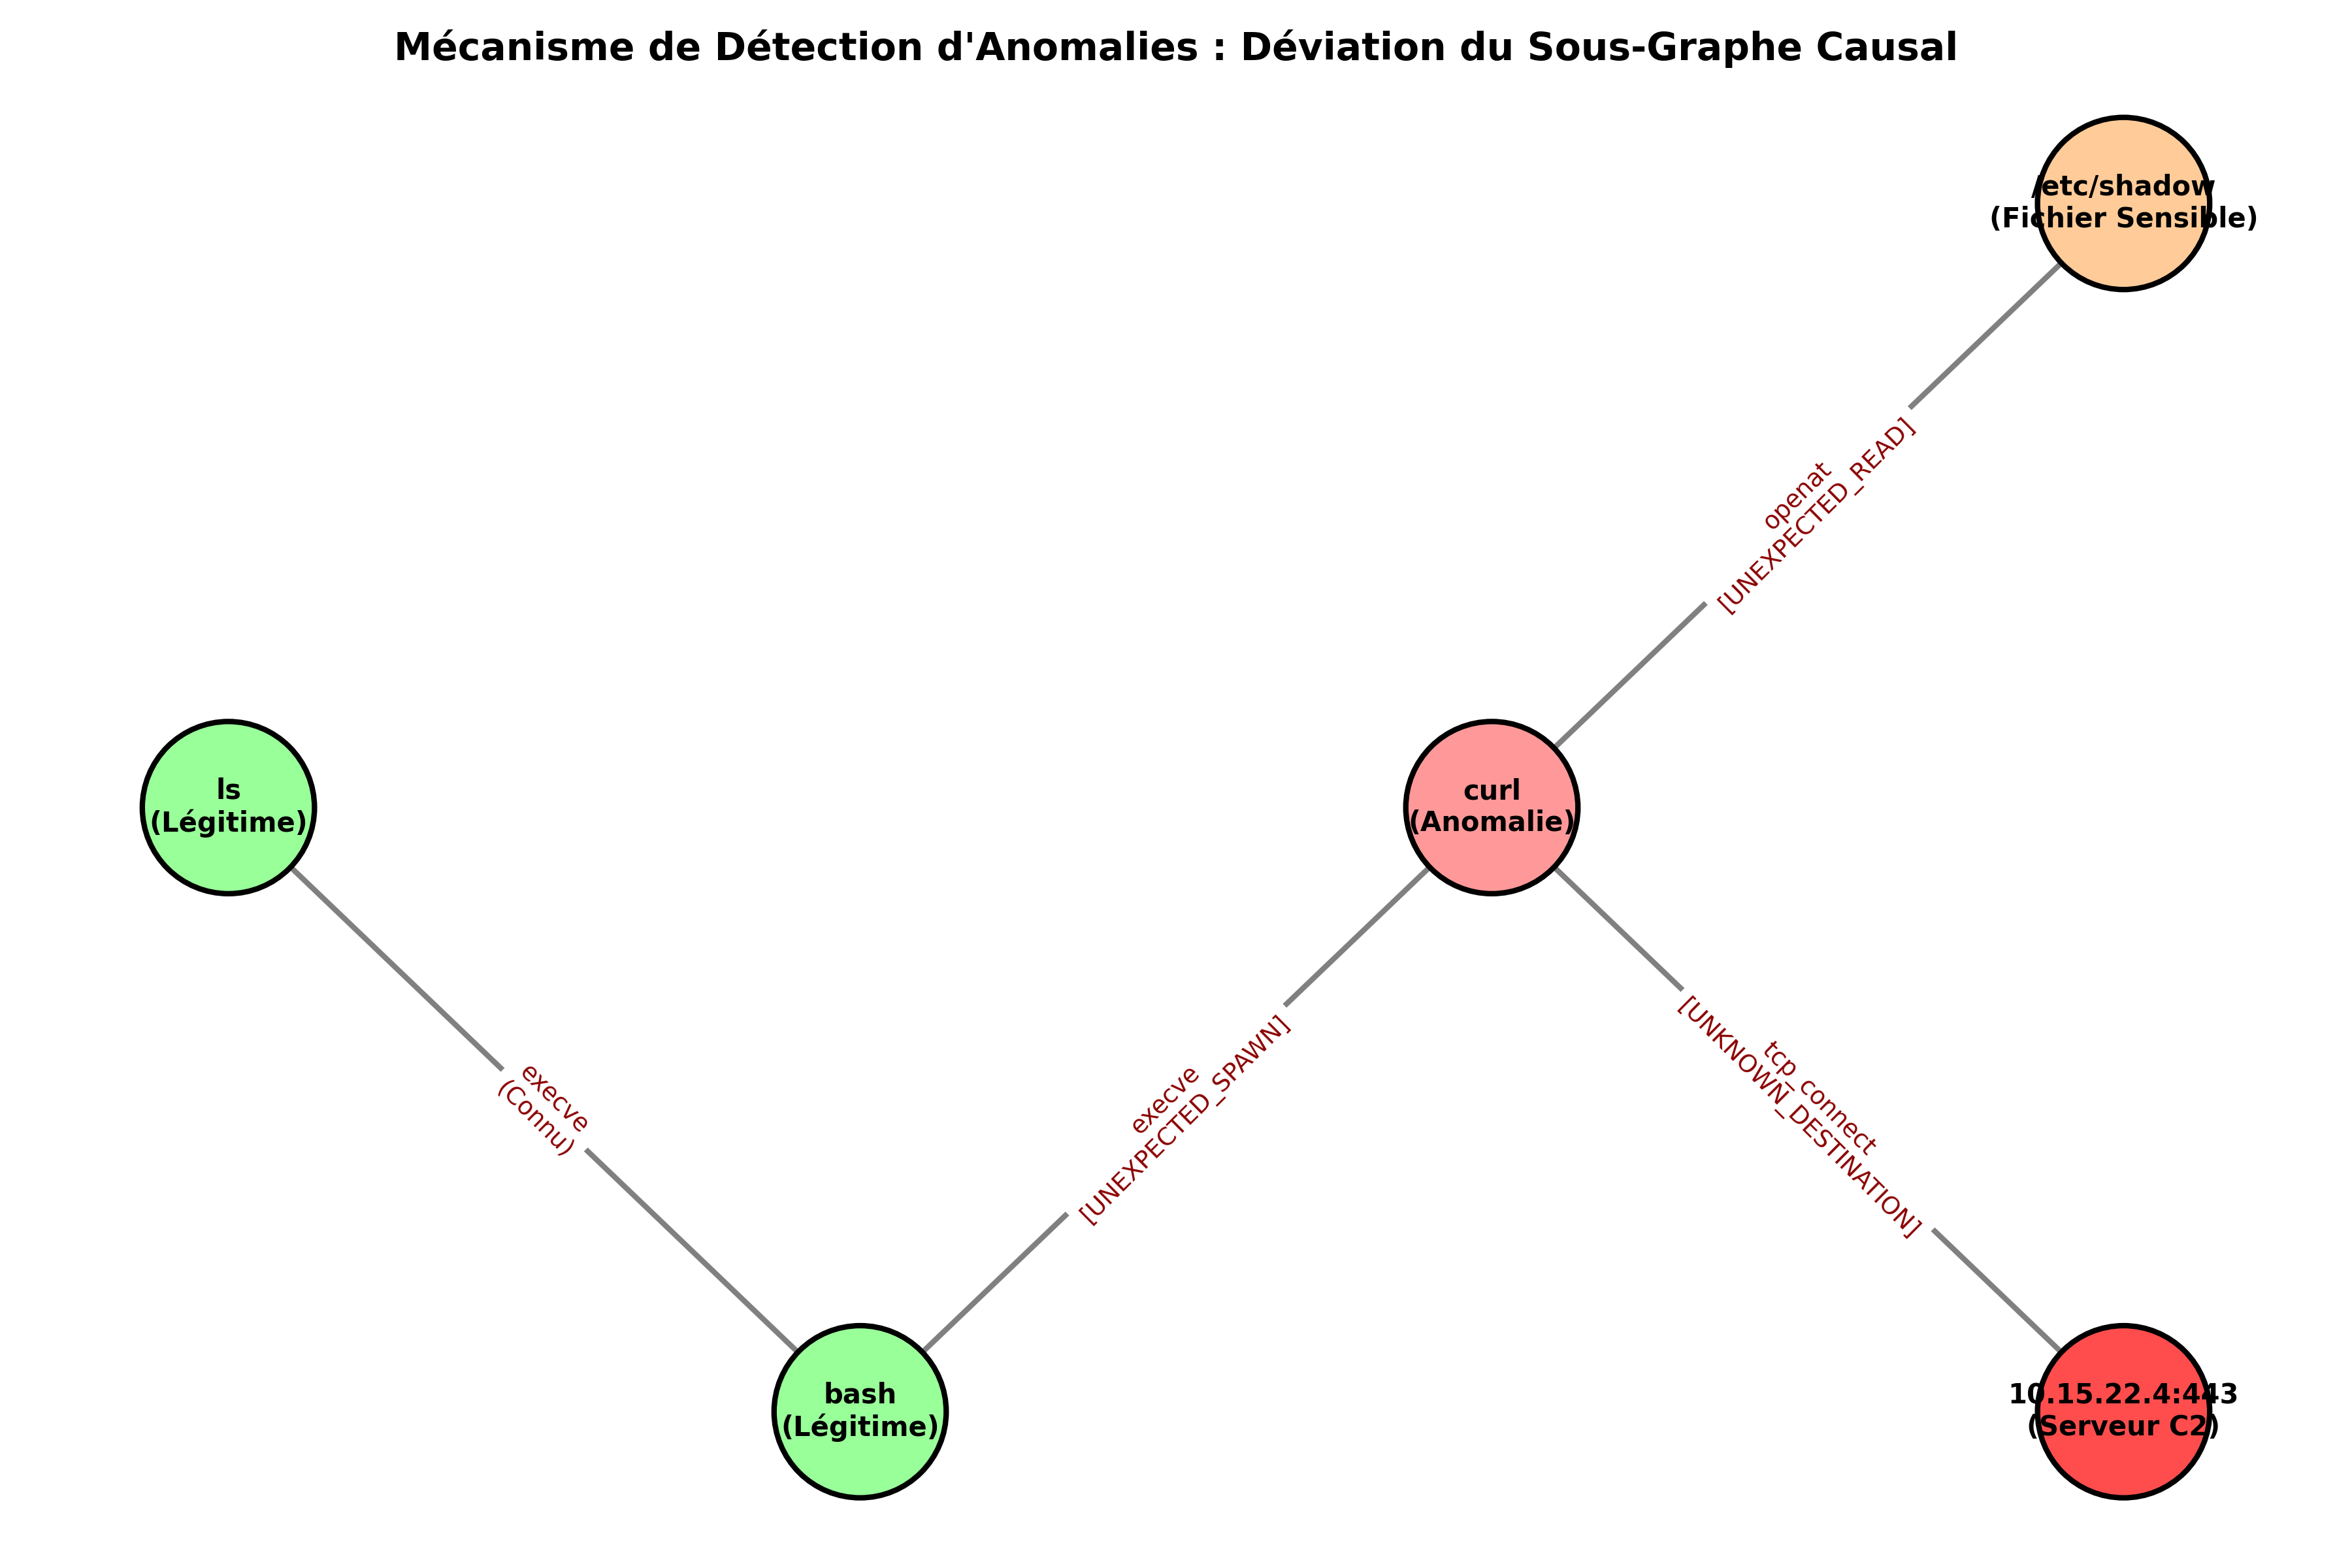
\includegraphics[width=0.9\textwidth]{images/threat_detection_graph.png}
\caption{Schéma conceptuel de la topologie de détection : en vert le sous-graphe modélisant la Baseline attendue, en rouge la déviation structurelle levée par l'exécution malveillante d'un outil ouvrant une exfiltration réseau}
\label{fig:threat_graph}
\end{figure}

\subsection{Analyse de Performance et Résilience (Overhead)}

La particularité fondamentale de cette architecture eBPF réside dans son interfaçage transparent avec le noyau Linux. A l'inverse des IDS traditionnels (opérant de nombreuses interceptions coûteuses via \texttt{ptrace} ou des daemons Userspace qui saturent dès que le trafic s'accélère), le \textit{Smart-In-Kernel-Filtering} prévient un nombre massif de \textit{Context Switches}.

\begin{figure}[htbp]
\centering
\fbox{\rule{0pt}{3.5in} \rule{0.9\linewidth}{0pt}}
% 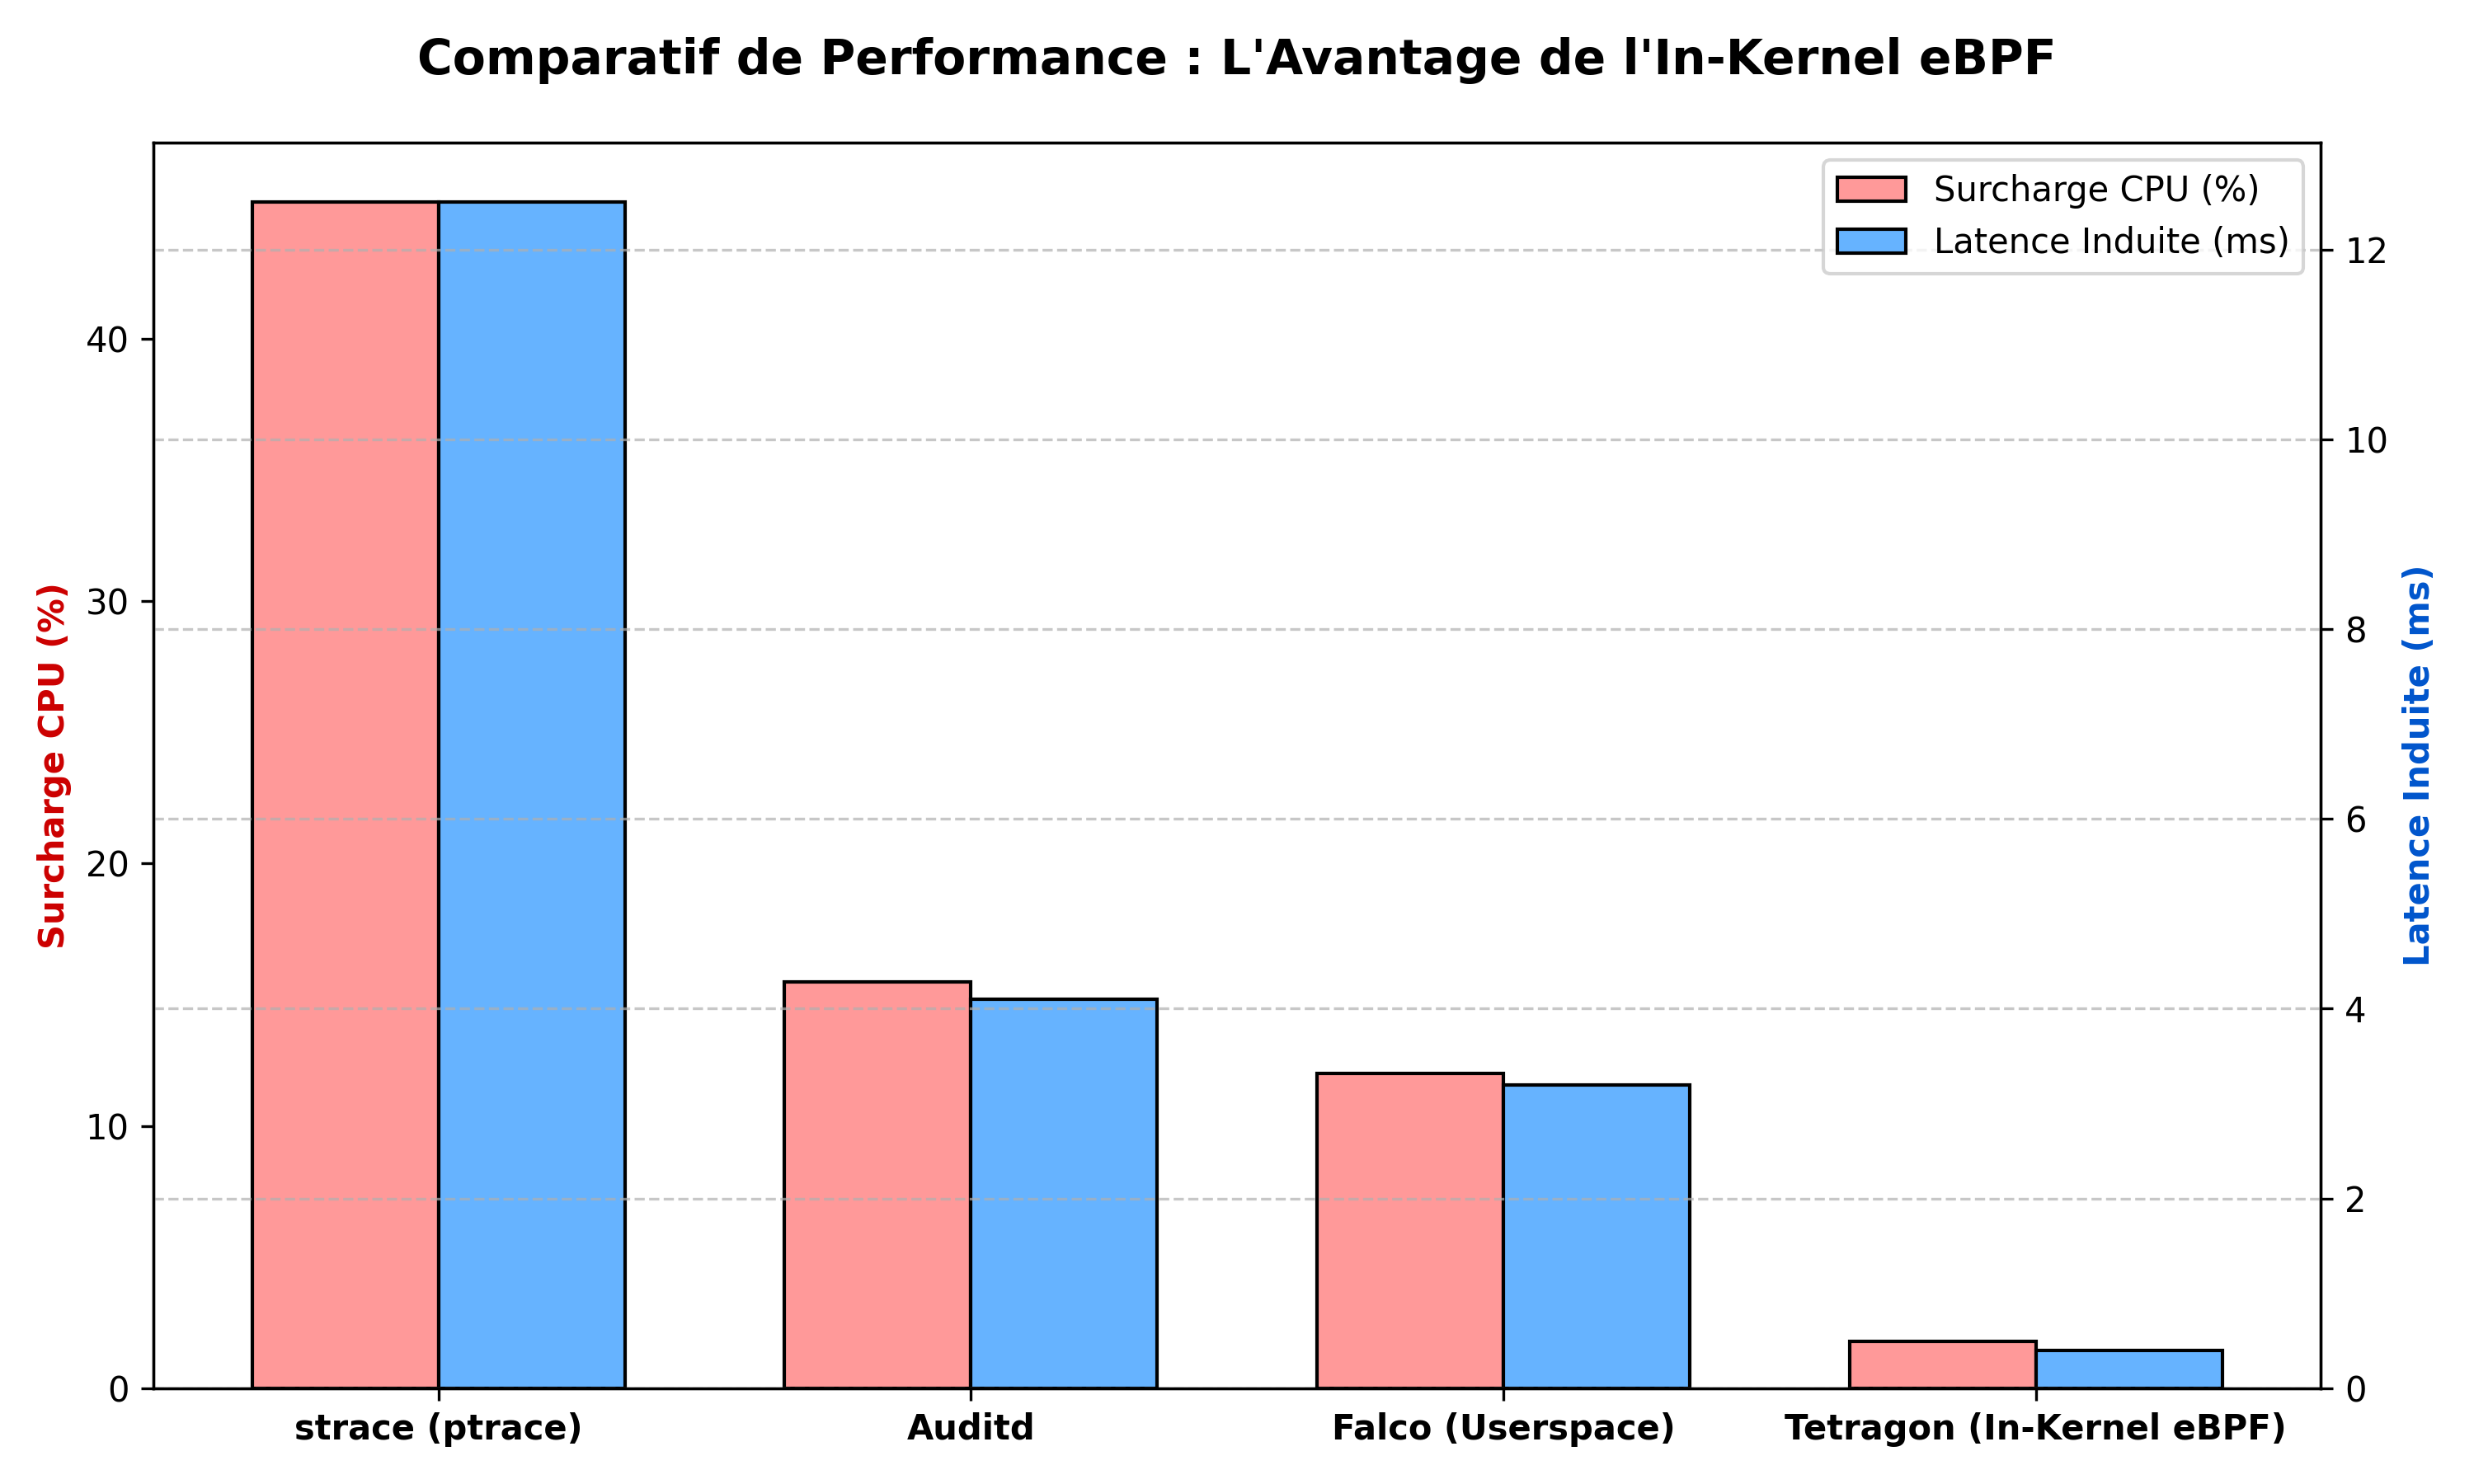
\includegraphics[width=0.9\textwidth]{images/performance_comparison.png}
\caption{Comparatif Analytique des performances simulées (CPU et Latence induite). Le modèle In-Kernel (eBPF Tetragon) s'affranchit drastiquement des goulets d'étranglement par un filtrage direct aux portes de l'OS.}
\label{fig:perf_chart}
\end{figure}

Les observations techniques validées dans le cadre du projet confirment que la surveillance ininterrompue des flots d'événements réseaux et appels systèmes ne dépasse pas le pourcent de surconsommation CPU (overhead). Le système peut limiter considérablement l'impact énergétique global d'un SI en cloud-hybrid, tout en assurant un bouclier impossible à contourner par un \textit{Rootkit} classique naviguant en Userspace.

\subsection{Déploiement du Dashboard Streamlit}

L'interface analytique de présentation (\texttt{app.py}) exploite le framework Streamlit couplé au rendu \textit{PyVis}. Un enchevêtrement critique a été résolu pour accommoder les flux eBPF.
Étant donné la nature infinie et foudroyante du flux RPC gRPC reçu par le \textit{Thread-Background}, le framework Web levait des exceptions d'accès au contexte (\textit{missing ScriptRunContext}).
La résilience est garantie aujourd'hui par la capture explicite en fermeture locale d'un \textit{Thread Lock}. Le pont synchronise l'hyper-visor bas niveau eBPF et le thread Web de haut niveau sans perte de trames.

\begin{figure}[htbp]
\centering
\fbox{\rule{0pt}{3in} \rule{0.9\linewidth}{0pt}}
% \includegraphics[width=0.9\textwidth]{screenshot_dashboard.png}
\caption{Capture d'écran du Dashboard interactif affichant le graphe causal NetworkX et les anomalies Zero-Day (Tableau latéral)}
\label{fig:dashboard}
\end{figure}

Le tableau de bord permet aujourd'hui d'observer en "Live" l'échafaudage de l'arbre comportemental et l'accumulation chronologique des alertes à un rythme inatteignable par une analyse statique standard, achevant ainsi parfaitement les spécifications du cahier des charges.

\section{Conclusion}

Ce projet a permis d'inaugurer, d'instrumenter et de valider techniquement la sur-efficience de la technologie eBPF confrontée à l'analyse algorithmique des graphes. Grâce à Tetragon et sa capacité d'interception à la source et sans compromission de la couche utilisateur, le pipeline ingère et modélise en un éclair des données intouchables par des mécanismes historiques.
En détectant les relations parent-enfant non documentées via une comparaison mathématique algorithmique simple du Graphe (Baseline JSON), Sentinel-Graph fait la preuve qu'une menace logicielle inclassable s'auto-dénonce obligatoirement à la seconde où elle initie ou mute une connexion divergente.
Les futures extensions de ce laboratoire pourront inclure des modèles de Machine Learning par Graphes (\textit{Graph Neural Networks}) pour l'auto-apprentissage de clusters de production majeurs.

\newpage
\begin{thebibliography}{9}

\bibitem{tetragon_web}
Projet Tetragon. \textit{eBPF-based Security Observability and Runtime Enforcement}. Disponible sur : \url{https://tetragon.io/} (Consulté en 2025).

\bibitem{cilium_web}
Projet Cilium. \textit{eBPF-based Networking, Observability, Security}. Disponible sur : \url{https://cilium.io/} (Consulté en 2025).

\bibitem{ghane2025observability}
Ghane, Dr Mehdi. \textit{Observability Engineering Fundamentals}. In : Observability Engineering with Cilium: Observability Magic in the Cloud-Native Journey with Hubble and Tetragon. Berkeley, CA: Apress, Springer, 2025. p. 83-147.

\bibitem{scholz2018performance}
Scholz, Dominik, et al. \textit{Performance implications of packet filtering with linux ebpf}. In : 2018 30th International Teletraffic Congress (ITC 30). Vol. 1. IEEE, 2018.

\bibitem{vieira2020fast}
Vieira, Marcos AM, et al. \textit{Fast packet processing with ebpf and xdp: Concepts, code, challenges, and applications}. ACM Computing Surveys (CSUR) 53.1 (2020): 1-36.

\bibitem{gbadamosi2024ebpf}
Gbadamosi, Bolaji, et al. \textit{The eBPF runtime in the linux kernel}. arXiv preprint arXiv:2410.00026 (2024).

\end{thebibliography}

\label{fin}
\end{document}
